\subsection*{4.4 Wellen}
    Höhe $\Phi$:
    \mathbox{\Psi (z, t) = A cos(\omega t - k z)}
    Wellenzahl $k = \frac{2 \pi}{\lambda}$, $z$ bezeichnet die entfernung zum Ursprung der cosinusfunktion zu Zeitpunkt $t_0$

    Phasengeschwindigkeit: Höhe konstant und somit Argument des cos() konstant:
    \mathbox{\omega t - k z = const}
    \mathbox{v_{ph} = c = f \lambda = \frac{\omega}{k}}
    Frequenz $f$

    Gruppengeschwindigkeit:
    \mathbox{v_{gr} = \frac{d \omega}{dk}}


    Intensität einer Welle: Energie
    Potentielle Energie:
    \mathbox{\Delta E_p = \int \vec{F} \vec{dx} = \frac{1}{2} D x_0^2 \text{mit} D = \omega^2 m}
    Kinetische Energie:
    \mathbox{\Delta E_k = \frac{1}{2} \Delta m v^2 \text{mit} v = \omega s}
    $\rightarrow \Delta E_p = \Delta E_k$  

    Energiestromdichte:
    \mathbox{\vec{j_E} = \frac{1}{A} \frac{\Delta E_k}{\Delta t} = \rho_E \vec{v_ph}}

    Reflektion von Wellen:
    Phasensprung bei Welle im Seil mittels Superposition mit einer Welle von der anderen Seite
    \centering
    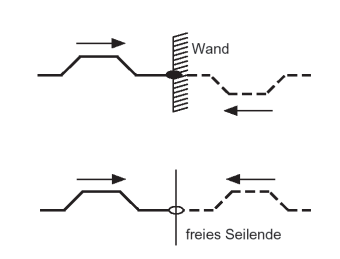
\includegraphics[height = 30mm]{src/images/welle_superposition.png}
